\chapter{统计数据的度量,概率分布,生成随机数}

Python 中的统计分析工具包 scipy.stats 包括80多个连续型随机分布以及10个离散型随机分布,结合 Numpy,Pandas 工具包,基本能满足统计分析的全部需要。

\section{统计数据的概括性度量}

统计数据的概括性度量主要包括:均值、方差、众数、中位数、偏度、峰度等。

\subsection{最大值、最小值、求和}

\subsection{均值、方差}

一组数据相加后除以数据的个数得到的结果称作均值。一般的均值可以用 numpy 中的 mean 方法求得:

\begin{lstlisting}[Language=Python]
>>> import numpy as np
>>> a = [5, 6, 16, 9]
>>> np.mean(a)
9.0
\end{lstlisting}

numpy 中的 average 方法不仅能求得简单平均数,也可以求出加权平均数。average 里面可以跟一个 weights 参数,里面是一个权数的数组,例如:

\begin{lstlisting}[Language=Python]
>>> np.average(a)
>>> 9.0
>>> np.average(a, weights = [1, 2, 1, 1])
>>> 8.4
\end{lstlisting}


计算方差时,可以利用 numpy 中的 var 函数,默认是总体方差(计算时除以样本数 N),若需要得到样本方差(计算时除以 N - 1),需要跟参数 ddo f= 1,例如

\begin{lstlisting}[Language=Python]
>>> import pnumpy as np
>>> a = [5, 6, 16, 9]
>>> np.var(a) # 计算总体方差
18.5

>>> np.var(a, ddof = 1) # 计算样本方差
24.666666666666668

>>> b = [[4, 5], [6, 7]]
>>> b
[[4, 5], [6, 7]]

>>> np.var(b) # 计算矩阵所有元素的方差
1.25

>>> np.var(b, axis = 0) # 计算矩阵每一列的方差
array([1., 1.])

>>> np.var(b, axis = 1) # 计算矩阵每一行的方差
array([0.25, 0.25])

\end{lstlisting}

计算标准差时,可以利用 numpy 中的 std 函数,使用方法与 var 函数很像,默认是总体标准差,若需要得到样本标准差,需要跟参数 ddof =1,

\begin{lstlisting}[Language=Python]
>>> import pnumpy as np
>>> a = [5, 6, 16, 9]
>>> np.std(a) # 计算总体标准差
4.301162633521313

>>> np.std(a, ddof = 1 ) # 计算样本标准差
4.96655480858378

>>> np.std(b) # 计算矩阵所有元素的标准差
1.118033988749895

>>> np.std(b, axis = 0) # 计算矩阵每一列的标准差
array([1., 1.])

>>> np.std(b, axis = 1) # 计算矩阵每一列的标准差
array([0.5, 0.5])

\end{lstlisting}



对于 pandas 的 DataFrame 类型,也可以用里面的 mean 函数可以求得所有行或所有列的平均数,例如:

\begin{lstlisting}[Language=Python]
>>> import pandas as pd
>>> df = pd.DataFrame(np.array([[85, 68, 90], [82, 63, 88], [84, 90, 78]]), columns=['统计学', '高数', '英语'], index=['张三', '李四', '王五'])
>>> df
统计学  高数  英语
张三   85  68  90
李四   82  63  88
王五   84  90  78

>>> df.mean() # 显示每一列的平均数

统计学    83.666667
高数     73.666667
英语     85.333333
dtype: float64

>>> df.mean(axis = 1) # 显示每一行的平均数
张三    81.000000
李四    77.666667
王五    84.000000
dtype: float64
\end{lstlisting}

若要得到某一行或某一列的平均值,则可以使用 iloc 选取改行或该列数据,后面跟 mean 函数就能得到,例如:

\begin{lstlisting}[Language=Python]
>>> df
    统计学  高数  英语
张三   85  68  90
李四   82  63  88
王五   84  90  78

>>> df.iloc[0, :].mean()  # 得到第 1 行的平均值
81.0

>>> df.iloc[:, 2].mean() # 得到第 3 列的平均值
85.33333333333333

\end{lstlisting}

pandas 中的 var 函数可以得到样本方差(注意不是总体方差),std 函数可以得到样本标准差,若要得到某一行或某一列的方差,则也可用 iloc 选取某行或某列,后面再跟 var 函数或 std 函数即可,例如:

\begin{lstlisting}[Language=Python]
>>> df.var() # 得到每一列的方差
统计学      2.333333
高数     206.333333
英语      41.333333
dtype: float64

>>> df.var(axis = 1) # 得到每一行的方差
张三    133.000000
李四    170.333333
王五     36.000000
dtype: float64

>>> df.std() # 得到每一列的标准差
统计学     1.527525
高数     14.364308
英语      6.429101
dtype: float64

>>> df.std(axis = 1) # 得到每一行的标准差
张三    11.532563
李四    13.051181
王五     6.000000
dtype: float64

>>> df.iloc[0, :].std() # 得到第 1 行的标准差
11.532562594670797

>>> df.iloc[:, 2].std() # 得到第 3 列的标准差
6.429100507328636
\end{lstlisting}

\subsection{中位数、分位数、众数}

使用 numpy 的 median 函数可以得到其中位数,quantile 函数可以得到其分位数,但numpy 包目前还没有计算众数的函数。例如:

\begin{lstlisting}[Language=Python]
>>> a = [8, 19, 34, 9, 18]
>>> np.median(a) # 得到数组 a 的中位数
18.0

>>> np.quantile(a, 0.25) # 得到数组 a 的上四分位数
9.0

>>> np.quantile(a, 0.5) # 得到数组 a 的中位数
18.0

>>> np.quantile(a, 0.75) # 得到数组 a 的下四分位数
19.0
\end{lstlisting}

pandas 可以使用 median,quantile,mode 函数分别计算中位数,分位数与众数。例如:

\begin{lstlisting}[Language=Python]
>>> df = pd.DataFrame(np.array([[85, 68, 90], [82, 63, 88], [84, 90, 88]]), columns=['统计学', '高数', '英语'], index=['张三', '李四', '王五'])
>>> df

    统计学  高数  英语
张三   85  68  90
李四   82  63  88
王五   84  90  88

>>> df.median() # 得到每一列的中位数
统计学    84.0
高数     68.0
英语     88.0
dtype: float64

>>> df.iloc[0, :].median() # 得到第一行的中位数
85.0

>>> df.quantile(0.25, axis = 1) # 得到所有行的上四分位数
张三    76.5
李四    72.5
王五    86.0
Name: 0.25, dtype: float64

>>> df.iloc[2, :].quantile(0.75) # 得到第三行的下四分位数
89.0

>>> df.mode()  # 得到所有列的众数
   统计学  高数    英语
0   82  63  88.0
1   84  68   NaN
2   85  90   NaN

\end{lstlisting}

\subsection{偏度、峰度}

在计算一个样本的偏度或峰度时,对于一般的数组类型,要用到统计分析工具包 scipy,对于 pandas 中的数据类型,可以调用 pandas 自带的计算偏度或峰度的函数。


\begin{lstlisting}[Language=Python]
>>> import scipy.stats as st
>>> a = [89, 23, 45, 18]

>>> st.skew(a) # 计算偏度
0.7565543738808015

>>> st.kurtosis(a) # 计算峰度
-1.0489580648783101
\end{lstlisting}


需要注意的是,pandas 计算峰度时需要至少 4 个数据。
\begin{lstlisting}[Language=Python]
>>> import pandas as pd
>>> import numpy as np
>>> df = pd.DataFrame(np.array([[85, 68, 90], [82, 63, 88], [84, 90, 78]]), columns=['统计学', '高数', '英语'], index=['张三', '李四', '王五'])
>>> df
    统计学  高数  英语
张三   85  68  90
李四   82  63  88
王五   84  90  78

>>> df.iloc[1, :].skew() # 计算第二行的偏度
-1.3294040702410526

>>> df.skew(axis = 0) # 计算所有列的偏度
统计学   -0.935220
高数     1.498959
英语    -1.545393
dtype: float64

>>> df.skew(axis = 1) # 计算所有行的偏度
张三   -1.373033
李四   -1.329404
王五    0.000000
dtype: float64

>>> df1 = pd.DataFrame(np.array([[85, 68, 90, 65], [82, 63, 88, 83], [84, 90, 78, 90], [72, 68, 91, 84]]), columns=['统计学', '高数', '英语', '计算机'], index=['张三', '李四', '王五', '马六'])
>>> df1
    统计学  高数  英语  计算机
张三   85  68  90   65
李四   82  63  88   83
王五   84  90  78   90
马六   72  68  91   84

>>> df1.kurt(axis = 0) # 计算 df1 所有列的偏度
统计学    3.090874
高数     3.365664
英语     3.090874
计算机    2.769386
dtype: float64

>>> df1.iloc[:, 2].kurt() #计算 df1 第 3 列的偏度
3.090874188966101
\end{lstlisting}

\section{概率密度、累计分布、逆函数}

计算概率分布的相关参数时,一般使用 scipy 包,常用的函数包括以下几个:

\begin{itemize}
  \item pdf:连续随机分布的概率密度函数
  \item pmf:离散随机分布的概率密度函数
  \item cdf:累计分布函数
  \item ppf:百分位函数(累计分布函数的逆函数)
  \item isf: 生存函数的逆函数(1 - cdf 的逆函数)
\end{itemize}

函数里面不仅能跟一个数据,还能跟一个数组。下面用正态分布举例说明:

\begin{lstlisting}[Language=Python]
>>> import scipy.stats as st

>>> st.norm.cdf(0) # 标准正态分布在 0 处的累计分布概率值
0.5

>>> st.norm.cdf([-1, 0, 1])# 标准正态分布分别在 -1, 0, 1 处的累计分布概率值
array([0.15865525, 0.5, 0.84134475])

>>> st.norm.pdf(0) # 标准正态分布在 0 处的概率密度值
0.3989422804014327

>>> st.norm.ppf(0.975)# 标准正态分布在 0.975 处的逆函数值
1.959963984540054

>>> st.norm.lsf(0.975)# 标准正态分布在 0.025 处的生存函数的逆函数值
1.959963984540054
\end{lstlisting}

对于非标准正态分布,通过更改参数 loc 与 scale 来改变均值与标准差:

\begin{lstlisting}[Language=Python]
>>> st.norm.cdf(0, loc=2, scale=1) # 均值为 2,标准差为 1 的正态分布在 0 处的累计分布概率值
0.022750131948179195
\end{lstlisting}

对于其他随机分布,可能更改的参数不一样,具体需要查官方文档。下面我们举一些常用分布的例子:

\begin{lstlisting}[Language=Python]
>>> st.binom.pmf(4, n=100, p=0.05) # 参数值 n=100, p=0.05 的二项分布在 4 处的概率密度值
0.17814264156968956

>>> st.geom.pmf(4, p=0.05) # 参数值 p=0.05 的几何分布在 4 处的概率密度值
0.04286875

>>> st.poisson.pmf(2, mu=3) # 参数值 mu=3 的泊松分布在 2 处的概率密度值
0.22404180765538775

>>> st.chi2.ppf(0.95, df=10) # 自由度为 10 的卡方分布在 0.95 处的逆函数值
18.307038053275146

>>> st.t.ppf(0.975, df=10) # 自由度为 10 的 t 分布在 0.975 处的逆函数值
2.2281388519649385

>>> st.f.ppf(0.95, dfn=2, dfd=12) # 自由度为 2, 12 的 F 分布在 0.95 处的逆函数值
3.8852938346523933
\end{lstlisting}


\section{标准化数据}

\section{生成随机数}

\subsection{用 Numpy 生成随机数}
在 python 中生成随机数有多种方法,首先可以用 Numpy 包的 random 函数生成随机数。例如,生成2 行 2 列, [1, 10] 内的均匀分布随机数:

\begin{lstlisting}[Language=Python]
>>> import numpy as np
>>> np.random.uniform(low=1, high=10, size=[2, 2])
array([[2.42454708, 5.54082358],
       [3.19289445, 3.4544002 ]])
\end{lstlisting}

生成一个正态分布的 2 行 2 列随机数,均值为 5, 标准差为 1:

\begin{lstlisting}[Language=Python]
>>> np.random.normal(loc=5, scale=1, size=[2,2])
array([[4.37643895, 6.00357154],
       [4.76599409, 4.64680265]])
\end{lstlisting}

生成一个泊松分布的 2 行 2 列随机数,均值为 5:

\begin{lstlisting}[Language=Python]
>>> np.random.poisson(mu=5, size=[2,2])
array([[3, 6],
       [7, 5]])
\end{lstlisting}


生成一个指数分布的 2 行 2 列随机数,均值为 5:

\begin{lstlisting}[Language=Python]
>>> np.random.exponential(scale=5, size=[2,2])
array([[3.14056456, 2.63627222],
       [5.44436781, 2.6088458 ]])
\end{lstlisting}

\subsection{用 Scipy 生成随机数}
另外一种生成随机数的方法是用 scipy 包不同分布函数自带的 rvs 生成随机数,例如,生成一个正态分布的 2 行 2 列随机数,均值为 5, 标准差为 1:

\begin{lstlisting}[Language=Python]
>>> import scipy.stats as st
>>> st.norm.rvs(loc=5, scale=1, size=[2,2])
array([[3.96964463, 4.14137383],
       [6.36342893, 3.99992325]])
\end{lstlisting}

生成一个指数分布的 2 行 2 列随机数,均值为 5:

\begin{lstlisting}[Language=Python]
>>> st.poisson.rvs(mu=5, size=[2,2])
array([[5, 7],
       [3, 9]])
\end{lstlisting}

\section{z 检验,t 检验, $\chi^2$ 检验}

 Python 中的假设检验一般用到 scipy 或 statsmodels 包,需要注意的是,这两个包里面各种检验的置信度都是 0.05。

\subsection{z 检验}

 对于大样本数据(样本量 $\geq$ 30),或者即使是小样本,但是知道其服从正态分布,并且知道总体分布的方差时,需要用 z 检验。在 python 中,由于 scipy 包没有 z 检验,我们只能用 statsmodels 包中的 ztest 函数。ztest 函数的一般用法在下页显示。

 \begin{table}[ht]
 \centering
 \caption{样本数据1} \label{tab:ztest}
 \begin{tabular}{|l|l|l|l|l|l|l|l|l|l|l|l|}
 \hline

 23 & 36 & 42 & 34 & 39 & 34 & 35 & 42 & 53 & 28 & 49 & 39 \\ \hline
 46 & 45 & 39 & 38 & 45 & 27 & 43 & 54 & 36 & 34 & 48 & 36 \\ \hline
 47 & 44 & 48 & 45 & 44 & 33 & 24 & 40 & 50 & 32 & 39 & 31 \\ \hline

 \end{tabular}
 \end{table}

 对于表格 \ref{tab:ztest} 的样本数据,检测其均值是否为 39, 该问题显然是一个双侧检验,由于样本个数大于 30,则使用 z 检验,python 代码如下:

 \begin{lstlisting}[Language=Python]
 >>> import statsmodels.stats.weightstats as sw
 >>> arr=[23,36,42,34,39,34,35,42,53,28,49,39,
 ... 46,45,39,38,45,27,43,54,36,34,48,36,
 ... 47,44,48,45,44,33,24,40,50,32,39,31]
 >>> sw.ztest(arr, value=39)
 (0.3859224924939799, 0.6995540720244979)
 \end{lstlisting}

 \begin{center}
 \begin{tcolorbox}[title = ztest 函数的语法]
 \textbf{ztest(x1, x2=None, value=0, alternative=`two-sided')}
 \tcblower
 \vspace{2pt}
 \begin{tcboutputlisting}
 \begin{tabular}{>{\bfseries}ll}
   输入参数:&\\
   x1 &数组,第一个样本的数据值\\
   x2 & 数组,第二个样本的数据值,默认没有值\\
   \specialrule{0em}{2pt}{2pt}
\multirow{2}*{value} &浮点型数值,若是单样本,则 value 是样本假设的均值,\\
&若是双样本,则 value是两个样本均值的差值\\
\specialrule{0em}{2pt}{2pt}
 \multirow{3}*{alternative}&字符串,备选假设 H1,默认为 two-sided',表示双侧检验,\\
 & 若为 `larger',备选假设 H1 大于 value 值\\
 & 若为 `smaller',备选假设 H1 小于 value 值\\
\specialrule{0em}{2pt}{2pt}
 返回值:&\\
 tstats & 统计量值\\
 pvalue & p 值
 \end{tabular}
 \end{tcboutputlisting}
 \tcbuselistingtext

  \end{tcolorbox}
  \end{center}


从 ztest 的运行结果可以看出,统计量值为 0.385,而 p 值是 0.699,在置信度 $\alpha=0.05$ 时,由于 p 值大于 $\alpha$,接受原假设,认为该样本的均值是 39。

若要检测该样本均值是否大于 39,即原假设 H0:$\mu>39$,备选假设为:$\mu\leq 39$,则我们需要在代码中增加一个参数 alternative=``smaller”:

\begin{lstlisting}[Language=Python]
>>> sw.ztest(arr, value=39, alternative="smaller")
(0.3859224924939799, 0.650222963987751)
\end{lstlisting}

检测结果的 p 值为 0.650,大于置信度 0.05,则接受原假设,认为样本均值大于39。假设另外一个样本 2 的数据:

\begin{table}[ht]
\centering
\caption{样本数据2}
\begin{tabular}{|l|l|l|l|l|l|l|l|l|l|}
\hline
41  & 34  & 36  & 32  & 32  & 35  & 33  & 31  & 35  & 34  \\ \hline
37  & 34  & 31  & 36  & 37  & 34  & 33  & 37  & 33  & 38  \\ \hline
38  & 37  & 34  & 36  & 36  & 31  & 33  & 36  & 37  & 35  \\ \hline
33  & 34  & 33  & 35  & 34  & 34  & 34  & 35  & 35  & 34 \\ \hline
\end{tabular}
\end{table}

检测两个样本的均值是否相等,因为两个样本都是大样本,使用 z 检验, python 代码如下:
\begin{lstlisting}[Language=Python]
>>> arr2 = [41, 34, 36, 32, 32, 35, 33, 31, 35, 34,
... 37, 34, 31, 36, 37, 34, 33, 37, 33, 38,
... 38, 37, 34, 36, 36, 31, 33, 36, 37, 35,
... 33, 34, 33, 35, 34, 34, 34, 35, 35, 34]
>>> sw.ztest(arr, arr2, value=0)
(3.775645601380307, 0.0001595937672736755)
\end{lstlisting}

从 ztest 的检验结果可以看出,p 值小于 0.05, 则拒绝原假设,认为两个样本的均值不相等。

\subsection{t 检验}
小样本(样本量小于30个),一般用 t 检验。对于 t 检验,可以根据样本特点,用 scipy 包中的 ttest\_1sample(单样本 t检验函数),ttest\_ind(两个独立样本的 t 检验),ttest\_rel (两个匹配样本的 t 检验)。但这些函数得到都是双侧 t 检验的 p 值。如果是单侧检验,我们还要进行一些换算,得到单侧检验的 p 值。

ttest\_1sample 函数的语法为:

\begin{center}
\begin{tcolorbox}[title = ttest\_1sample 函数的语法]
\textbf{ttest\_1samp(a, popmean)}
\tcblower
\vspace{2pt}
\begin{tcboutputlisting}
\begin{tabular}{>{\bfseries}ll}
  输入参数:&\\
  a &数组,样本的数据值\\
  popmean & 原假设 $H_0$ 中样本的期望值\\
\specialrule{0em}{2pt}{2pt}
返回值:&\\
statistic & 统计量值\\
pvalue & 双侧检验的 p 值
\end{tabular}
\end{tcboutputlisting}
\tcbuselistingtext
\end{tcolorbox}
\end{center}

下面是一个样本的数据:
\begin{equation}
  99.3\quad 98.7\quad 100.5\quad 101.2\quad 98.3\quad 99.7\quad 99.5\quad 102.1\quad 100.5\nonumber
\end{equation}

检测样本均值是否等于100,对其进行双侧 t 检验的语法为:

\begin{lstlisting}[Language=Python]
>>> import scipy.stats as st
>>> a = [99.3, 98.7, 100.5, 101.2, 98.3, 99.7, 99.5, 102.1, 100.5]
>>> st.ttest_1samp(a, 100)
Ttest_1sampResult(statistic=-0.054996133220328265, pvalue=0.9574902045208937)
\end{lstlisting}

从结果可以看出,双侧检验的 p 值为 0.95, 大于置信度 0.05,因此接受原假设,认为样本的均值是100。若是单侧检验中的左侧检验,则 p 值为 $0.957/2=0.4785$,若是右侧检验,则 p 值为 $1-0.957/2=0.5215$。

假设有另外一个样本的数据:
\begin{equation}
91.1\quad 93.7\quad 93.6\quad 96.1\quad 94.3\quad
       92.2\quad 94.0\quad 95.7\quad 97.1 \nonumber
\end{equation}

若两个样本相互独立,检测两个样本的均值是否相等,使用 ttest\_ind 函数。

\begin{center}
\begin{tcolorbox}[title = ttest\_ind 函数的语法]
\textbf{ttest\_ind(a, b, axis=0, equal\_var=True) }
\tcblower
\vspace{2pt}
\begin{tcboutputlisting}
\begin{tabular}{>{\bfseries}ll}
  输入参数:&\\
  a &数组,样本1的数据值\\
  b &数组,样本2的数据值\\
  axis & 一般为 0\\
  \multirow{2}{*}{equal\_var} & 若为 true,表示两个样本由相同的方差\\
  &若为 false,表示两个样本的方差不同,使用合并方差\\
\specialrule{0em}{2pt}{2pt}
返回值:&\\
statistic & 统计量值\\
pvalue & 双侧检验的 p 值
\end{tabular}
\end{tcboutputlisting}
\tcbuselistingtext
\end{tcolorbox}
\end{center}

假设两个样本的方差不同,则独立双样本的 t 检验 python 代码为:

\begin{lstlisting}[Language=Python]
>>> import scipy.stats as st
>>> a = [99.3, 98.7, 100.5, 101.2, 98.3, 99.7, 99.5, 102.1, 100.5]
>>> b = [91.1, 93.7, 93.6, 96.1, 94.3, 92.2, 94.0, 95.7, 97.1]
>>> st.ttest_ind(a, b, equal_var = False)
Ttest_indResult(statistic=7.723221821038956, pvalue=2.4331092243754622e-06)
\end{lstlisting}

从上面结果可以看出,p 值小于置信度 0.05,拒绝原假设,认为两个两个样本的均值不同。

若两个样本是匹配样本,使用函数 ttest\_rel,它的语法更简单,只需在函数里输入两个样本的数组即可。假设上面两个样本为匹配样本,python 代码为:

\begin{lstlisting}[Language=Python]
>>> import scipy.stats as st
>>> a = [99.3, 98.7, 100.5, 101.2, 98.3, 99.7, 99.5, 102.1, 100.5]
>>> b = [91.1, 93.7, 93.6, 96.1, 94.3, 92.2, 94.0, 95.7, 97.1]
>>> st.ttest_rel(a, b)
Ttest_relResult(statistic=10.845107419335658, pvalue=4.617509769582176e-06)
\end{lstlisting}

结果显示,p 值小于置信度 0.05,拒绝原假设,认为这两个匹配样本的均值不同。

\chapter{方差分析}

方差分析用于研究一个或多个分类型自变量与一个数值型因变量之间的关系,即检测多个总体的均值是否相等,一般要使用 F 检验。

\section{单因素方差分析}

\subsection{使用 scipy 的 f\_oneway 函数}
对于单因素方差分析, 其中一个方法是使用 scipy 包提供了 f\_oneway 函数。

例如了调查了三个行业的投诉次数,希望分析行业类别对投诉次数是否有影响。各样本的数据如下所示:
\begin{align}
  \text{零售业:}&57~~ 66~~ 49~~ 40~~ 34~~ 53~~ 44\nonumber\\
  \text{旅游业:}&68~~ 39~~ 29~~ 45~~ 56~~ 51\nonumber\\
  \text{制造业:}&44~~ 51~~ 65~~ 77~~/+ 58\nonumber
\end{align}

使用 f\_oneway 函数做单因素方差分析 F 检验的 python 代码为:

\begin{lstlisting}[Language=Python]
>>> import scipy.stats as st
>>> a = [57, 66, 49, 40, 34, 53, 44]
>>> b = [68, 39, 29, 45, 56, 51]
>>> c = [44, 51, 65, 77, 58]
>>> st.f_oneway(a, b, c)
F_onewayResult(statistic=1.3141307534447377, pvalue=0.29792936408490506)
\end{lstlisting}

从结果可以看出, p 值大于 0.05,则可以认为在 95\% 的置信度内接受愿家人,认为行业类别对投诉次数没有影响。

\subsection{使用 statsmodels 的 anova\_lm 函数}
若想要更详细的方差分析结果,或者多个因素的方差分析,就要使用 statsmodels 包了,statsmodels 包常常结合 pandas 包一起使用。例如,下面的数据存储在 complainNumber.xlsx 的 excel 文件中,

\begin{figure}[ht]
  \centering
  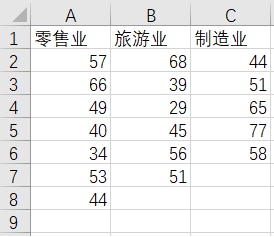
\includegraphics{figure/chapter3/complain.png}
\end{figure}

在做方差分析时,我们需要转化成因变量对应自变量的形式,即将上面的数据转化为下面的形式:

\begin{figure}[ht]
  \centering
  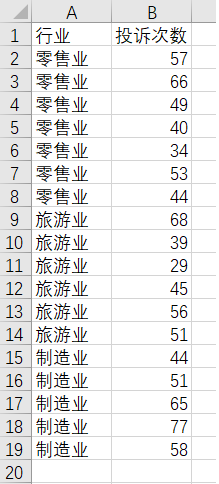
\includegraphics{figure/chapter3/complain2.png}
\end{figure}

通过 excel 转化好形式后,我们再导入到 pandas 数据库中。

\begin{lstlisting}[Language=Python]
>>> df = pd.read_excel(r'D:\Users\chen_\git\Statistics-book\datas\complainNumber.xlsx')
>>> df.head()
    行业  投诉次数
0  零售业    57
1  零售业    66
2  零售业    49
3  零售业    40
4  零售业    34
\end{lstlisting}

对于数据 df,我们首先将它放进 statsmodels 中的 OLS 模型里。OLS (ordinary least squares) 表示普通最小二乘模型,在统计分析中经常使用。该模型的建模模仿了 R 语言, 使用 pasty 语言的语法描述统计学公式。 python 代码如下:

\begin{lstlisting}[Language=Python]
>>> import statsmodels.formula.api as sm
>>> model = sm.ols(formula = '投诉次数 ~ C(行业)', data = df).fit()
\end{lstlisting}

其中,formula = `投诉次数 ~ C(行业)' 表示了单因素方差分析的统计学公式, \textasciitilde 左边的投诉次数为因变量,\textasciitilde 右边表示自变量,C 是 category 的缩写,表示行业是分类变量。

建立统计学模型后,再使用 anova\_lm 函数进行方差分析:

\begin{lstlisting}[Language=Python]
>>> from statsmodels.stats.anova import anova_lm
>>> model = sm.ols(formula = '投诉次数 ~ C(行业)', data = df).fit()
>>> result = anova_lm(model)
>>> print(result)
            df       sum_sq     mean_sq         F    PR(>F)
C(行业)      2.0   398.444444  199.222222  1.314131  0.297929
Residual  15.0  2274.000000  151.600000       NaN       NaN

\end{lstlisting}

上面的结果与 scipy 的 f\_oneway 函数的分析结果一致。

\section{双因素方差分析}

对于双因素方差分析,可以分为有交互作用的双因素方差分析和没有交互作用的双因素方差分析,假如有下面的数据,表示不同地区不同品牌的销量,由于是一一对应的数据,这个数据表是没有交互作用的双因素方差分析。


\begin{figure}[ht]
  \centering
  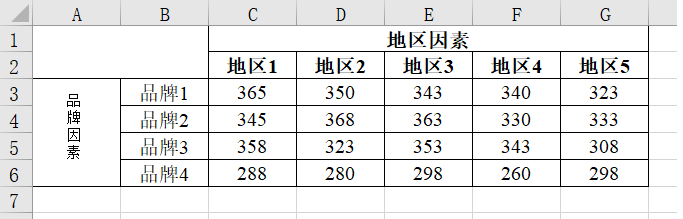
\includegraphics[scale=0.8]{figure/chapter3/twoFactor.png}
\end{figure}

我们首先将其转化为因变量对应自变量的形式:

\begin{figure}[ht]
  \centering
  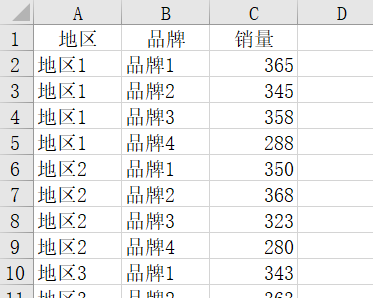
\includegraphics[scale=0.8]{figure/chapter3/twoFactor2.png}
\end{figure}

用 pandas 读取数据:

\begin{lstlisting}[Language=Python]
>>> df = pd.read_excel(r'D:\Users\chen_\git\Statistics-book\datas\twoFactorANOVA.xlsx')
>>> df.head()
    地区   品牌   销量
0  地区1  品牌1  365
1  地区1  品牌2  345
2  地区1  品牌3  358
3  地区1  品牌4  288
4  地区2  品牌1  350
\end{lstlisting}

构建 OLS 模型:

\begin{lstlisting}[Language=Python]
>>> model = sm.ols(formula = '销量 ~ C(地区) + C(品牌)', data = df).fit()
\end{lstlisting}

formula = `销量 ~ C(地区) + C(品牌)' 表示了无交互作用的双因素方差分析的统计模型。调用 anova\_lm 函数进行方差分析:

\begin{lstlisting}[Language=Python]
>>> result = anova_lm(model)
>>> print(result)
            df    sum_sq      mean_sq          F    PR(>F)
C(地区)      4.0   2011.70   502.925000   2.100846  0.143665
C(品牌)      3.0  13004.55  4334.850000  18.107773  0.000095
Residual  12.0   2872.70   239.391667        NaN       NaN
\end{lstlisting}

从上面结果可以看出, 地区的 p 值大于 0.05,说明地区对销量没有影响;而品牌的 p 值小于 0.05,说明品牌因素对销量有影响。

若对于同样的地区和品牌,有多个数据,则可能存在交互因素,例如下面的数据可能存在交互作用:

\begin{figure}[ht]
  \centering
  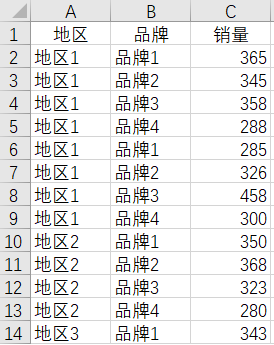
\includegraphics[scale=0.8]{figure/chapter3/twoFactor3.png}
\end{figure}


在构建统计模型时,需要改一下表达式:

\begin{lstlisting}[Language=Python]
>>> model = sm.ols(formula = '销量 ~ C(地区) + C(品牌) + C(地区):C(品牌)', data = df).fit()
\end{lstlisting}

调用 anova\_lm 函数生成结果:

\begin{lstlisting}[Language=Python]
>>> result = anova_lm(model)
>>> print(result)
               df        sum_sq      mean_sq         F    PR(>F)
C(地区)         4.0   2625.375000   656.343750  0.310603  0.858125
C(品牌)         3.0  16654.166667  5551.388889  2.627099  0.186915
C(地区):C(品牌)  12.0   9516.458333   793.038194  0.375292  0.915657
Residual      4.0   8452.500000  2113.125000       NaN       NaN
\end{lstlisting}

从 p 值可以看出,两个因素以及他们的交互作用对销量都没有影响。


\section{多元方差分析}
